\documentclass[11pt]{beamer}
\usepackage[utf8]{inputenc}
\usepackage[T1]{fontenc}
\usetheme{Warsaw}
\begin{document}
	
	%\setbeamercovered{transparent}
	%\setbeamertemplate{navigation symbols}{}
	
	
	\begin{frame}[plain]
	%empty frame
	\end{frame}
	
	\setbeamerfont{title}{size={\fontsize{28}{28}}}
	\title{\textbf{Hi}}
	\author{}
	\begin{frame}[plain]
	\maketitle
	\end{frame}

	\author{Rachana-PH15B007\\Guide: Prof. Arul Lakshminarayan}
	\setbeamerfont{title}{size=\large}
	\title{Entanglement Dynamics in a Randomly-Kicked Ising model}
	%\subtitle{}
	%\logo{}
	\institute{Department of Physics\\ Indian Institute of Technology Madras}
	\date{}
	\subject{Mini Project Jan-May 2019}
	\begin{frame}[plain]
	\maketitle
	\end{frame}



\begin{frame}
\frametitle{Kicked Ising model}
The Hamiltonian for a 1D transverse field kicked Ising model is: 

\begin{equation}\label{key}
H(t)= \sum_{j=1}^{L}\sigma_{j}^{x} \sigma_{j+1}^{x} + \sum_{k=-\infty}^{\infty}\delta(k-\dfrac{t}{T})\sum_{j=1}^{L}\sigma_{j}^{z}
\end{equation}
\end{frame}


\begin{frame}{Floquet Operator}
\begin{equation}
U = \exp(-iT\sum_{j=1}^{L}\sigma_{j}^{x} \sigma_{j+1}^{x})  \exp(-iT\sum_{j=1}^{L}\sigma_{j}^{z})
\end{equation}
\end{frame}


\begin{frame}{Floquet Operator \cite{PhysRevA.91.022318}}
 \begin{equation}
U = \exp(-i\dfrac{\pi}{4}\sum_{j=1}^{L}\sigma_{j}^{x} \sigma_{j+1}^{x})  \exp(-i\dfrac{\pi}{4}\sum_{j=1}^{L}\sigma_{j}^{z})
\end{equation}
\end{frame}

\begin{frame}{Entanglement Entropy\cite{PhysRevA.91.022318}}
\begin{figure}
	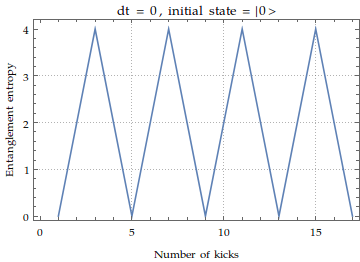
\includegraphics[scale=0.5]{dt0.png}
	\caption{Starting with the initial state $|0\rangle$ in a 8-spin chain, entanglement entropy of the subsystem consisting of first 4 spins is being plotted with time for dt = 0 }
	\label{normal}
\end{figure}
\end{frame}

\begin{frame}{Jordan Wigner Transformations}
Express the system in Fermion-momentum basis:

\begin{align}
H_{kick} &= 2 \Sigma_{k}  [d_{k}^\dagger d_{k} - d_{-k}^\dagger d_{-k}]\\
H_{after} &= -2\Sigma_{k}(  \cos k [d_{k}^\dagger d_{k} - d_{-k}^\dagger d_{-k}] -  \sin k [d_{-k}d_{k} + d_{k}^\dagger d_{-k}^\dagger])
\end{align}		

\end{frame}

\begin{frame}{Need for further simplification}

Define a new space whose basis states are $ |0\rangle $  and $ d_{k}^\dagger d_{-k}^\dagger |0\rangle $.

\begin{align}
H_{kick} &= -2 \Sigma_{k}  \sigma_{k}^z\\
H_{after} &= 2\Sigma_{k} (\cos k \sigma_{k}^z - \sin k \sigma_{k}^x )
\end{align}	
\end{frame}

\begin{frame}{Floquet Operator Now}

	\begin{align}
U_{kick}& = \exp(2 i T  \Sigma_{k}  \sigma_{k}^z)\\
U_{after} & = \exp(-2iT \Sigma_{k} (\cos k \sigma_{k}^z - \sin k \sigma_{k}^x))
\end{align}

\end{frame}

\begin{frame}{Very Simple Floquet operator!}
When $ T = \pi/4 $,

	\begin{equation}\label{key}
U = - \prod_{\otimes k} (\cos k + i \sin k \sigma_{k}^y)
\end{equation}

\end{frame}

\begin{frame}{Random protocol\cite{PhysRevB.98.064305}}
\begin{align*}
U_{n} & = U_{\text{after}}(U_{\text{kick}})^{\alpha_n} , \qquad  \alpha_n \epsilon \{0,1\}\\
\end{align*}
\end{frame}


\begin{frame}{Evolution on the Bloch sphere}
Consider a single k-mode:

\begin{align}
\begin{bmatrix}
v_{k}(t)\\u_{k}(t)
\end{bmatrix}  & = e^{i\beta} \cos[\dfrac{\theta}{2}] |0\rangle + e^{i\alpha} \sin[\dfrac{\theta}{2}] |1\rangle \\
&=   e^{i\beta}(\cos[\dfrac{\theta}{2}] |0\rangle + e^{i(\alpha-\beta)} \sin[\dfrac{\theta}{2}] |1\rangle)
\end{align}

\end{frame}


\begin{frame}{Evolution on the Bloch sphere, $ T = \pi/4 $}
	\begin{figure}[h]
	\centering
	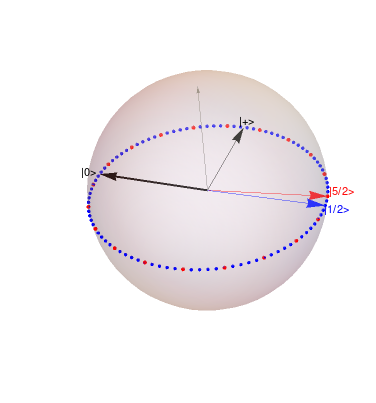
\includegraphics[width=0.55\linewidth]{piby4blochsphere}
	\caption{k-mode evolution, when  $T = \pi/4 $. The colored arrow shows the initial states for two modes $ k  = \pi/100 $ and $ k = 5\pi/100 $ }
	\label{fig:piby4blochsphere}
\end{figure}
\end{frame}

\begin{frame}{Evolution on the Bloch sphere, $ T = \pi/4 + 0.01 $}
	\begin{figure}
	\centering
	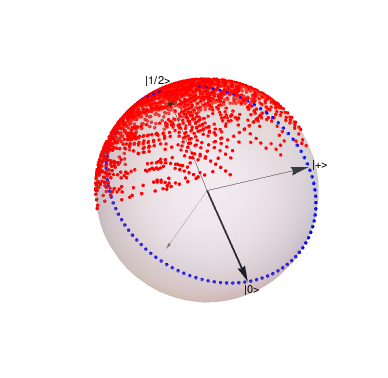
\includegraphics[width=0.5\linewidth]{blochsphere_half_01}
	\caption{k-mode evolution, when  $T = \pi/4 + 0.01 $ shown  in red for  $ k  = \pi/100 $ and the blue points correspond to $ T = \pi/4 $}
	\label{fig:blochspherehalf01}
\end{figure}
\end{frame}

\begin{frame}{Evolution on the Bloch sphere, $ T = \pi/4 + 0.01 $}
	\begin{figure}
	\centering
	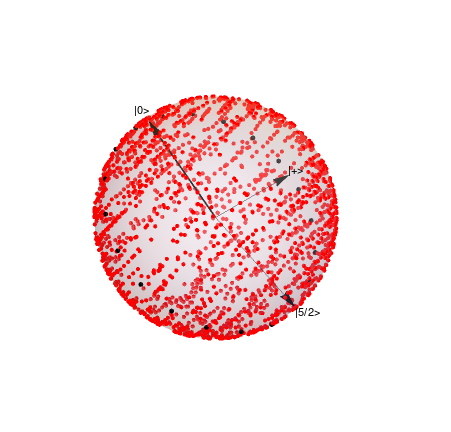
\includegraphics[width=0.5\linewidth]{blochsphere_fiveby2_01}
	\caption{k-mode evolution, when  $T = \pi/4 + 0.01 $ shown  in red for  $ k  = 5\pi/100 $ and the blue points correspond to $ T = \pi/4 $}
	\label{fig:blochspherefiveby201}
\end{figure}
\end{frame}

\begin{frame}{Entanglement entropy}
Von Neumann entropy:
\begin{equation}\label{key}
\mathcal{S} = - \rho \log\rho
\end{equation}

This is equivalent to the entropy of the eigen values of the correlation matrix given by\cite{Peschel_2003}\cite{Peschel_2009}:
\begin{equation}\label{key}
\mathcal{C} = \begin{bmatrix}
I - C & F\\
F^\dagger & C\\
\end{bmatrix} \text{where,} \quad C_{mn} = \langle c_m^\dagger c_{n}\rangle\, \text{and} \, F_{mn}  = \langle c_m^\dagger c_{n}^\dagger\rangle
\end{equation}



\end{frame}



\begin{frame}{Entanglement entropy}{Random case}
\begin{figure}
	\centering
	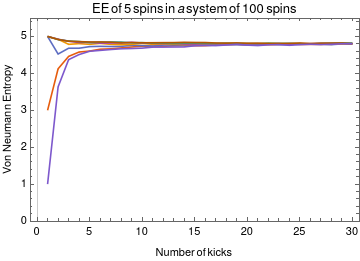
\includegraphics[width=0.7\linewidth]{5_95_EE}
%	\caption{}
	\label{fig:595ee}
\end{figure}

\end{frame}

\begin{frame}{Entanglement entropy}{Random case}
\begin{figure}
	\centering
	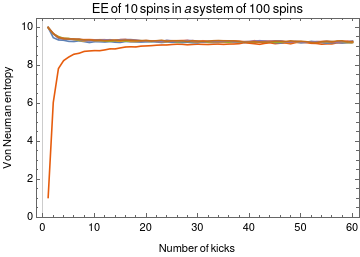
\includegraphics[width=0.7\linewidth]{10_90_EE}
%	\caption{}
	\label{fig:1090ee}
\end{figure}

\end{frame}

\begin{frame}{Remarks}
\begin{itemize}
	\item Special properties of $ T = \pi/4 $ has been previously explored for the periodic case \cite{PhysRevA.91.022318}. Special behaviour in aperiodic dynamics could lead to better understanding of the system
	\item Thermalization of aperiodic systems as shown in \cite{PhysRevX.7.031034} is not complete as we have seen an exceptional case. 
	\item Further studies of Thue Morse/Fibonacci sequenced protocols can show interesting results 
\end{itemize}
\end{frame}

\begin{frame}[allowframebreaks]{References}

\bibliographystyle{plain}
\bibliography{referencesforppt}

\end{frame}

\begin{frame}
\centering
Thank you!
\end{frame}

\end{document}